%!TEX root = ../document.tex
\chapter{Introduction}
In this master thesis we will look at how students can use a plant monitoring system called Monoplant to support their scientific inquiry when learning about photosynthesis. 

Computer based technology are increasingly being used for educational purposes, both in school settings and student-initiated settings. As of 2009 every high school student in Norway should have a personal computer available for use (UDIR). The use of ICT is receiving increased attention as it is believed that it can enhance students learning and provide productive learning environments. One important point is that the usage of ICT is important in itself to prepare students for working with technology. However, making use of the opportunities these technologies give us, by applying digital content specifically designed for educational contexts, is in our opinion of equal importance. 

With the advent of Internet connected embedded devices we feel that there is an opportunity to  distribute time consuming and tedious tasks to computers. By using digital sensors, quantitative data readings from our surroundings can be collected automatically. These data can then be used to promote student reflection and conceptual knowledge building of difficult scientific concepts such as photosynthesis. 

\section{Motivations and background}
When we started working with ideas for this thesis, our goal was to do research on an actual product in a real world setting. As we chose to develop a system ourselves, a major part of the work on this thesis became to build and complete the system. In 2012 during a project in inf5261 - \emph{Development of mobile information systems} we developed a mixed reality game called Plantagotchi. The prototype developed in this course became the foundation of the system in this thesis referred to as Monoplant. The idea was to animate a digital version of a real plant, which was affected by how the real plant was treated. In this project the user group was children at the age 8-12 and the game was planned to be used as a school contest where classes competed in getting the happiest plant. The educational outcome being pupil motivation for learning about growth conditions for plants, so that they could win the game. 

\begin{figure}
\centering
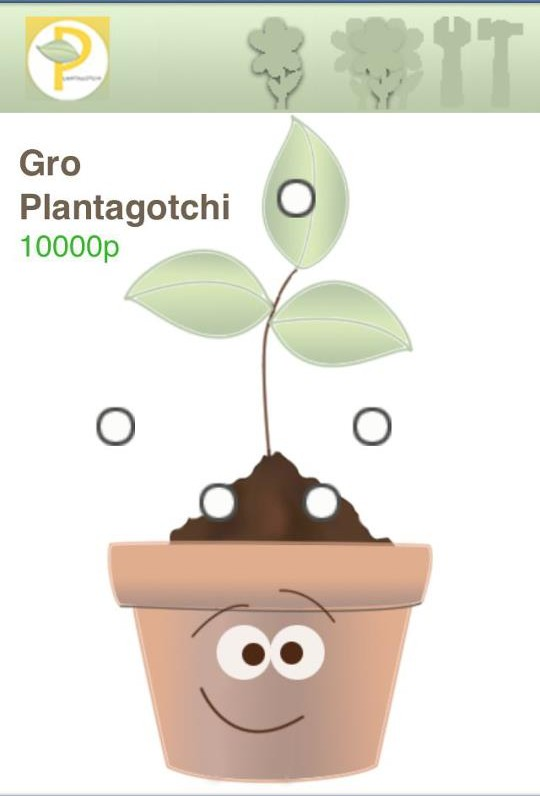
\includegraphics[width=0.3\textwidth]{img/introduction/plantagotchi.jpg}
\caption{Screenshot of Plantagotchi prototype}
\label{fig:scrshotplantagotchi}
\end{figure}

During the spring of 2013 we both took the course inf5790 \emph{Technology enhanced learning} and were introduced to the field of Computer Supported Collaborative Learning (CSCL). As we brought with us an idea of an application which pupils could use to collaboratively learn about a scientific domain, CSCL became the field where we could adapt theoretical perspectives and concepts which set words and explained our personal ideas and experiences. 

As mentioned, the starting point of this thesis was to do research on an actual working system, in an authentic environment. We therefore brought with us the ground idea from Plantagotchi and spent a lot of time improving it and developing a new working prototype. This meant that when we in October 2013 got in touch with a school, we had a fully working plant monitoring system which we could test with it's intended users in their natural setting. The focus in this thesis is therefore directed to this case study performed in a high school biology class. We will however provide some background information about the decisions made while developing Monoplant. 

\section{Monoplant}
Plants live a slow life, they grow slowly and move slowly. Humans have no means of directly observe when a plant grow, but we are able to see that it has grown or bloomed. However, humans have the ability to use tools in order to make sense of the world, and we have created such a tool: Monoplant, which can help us see how plants evolve over time.

Monoplant is a monitoring system for plants. It consists of three parts: 1) a plant station with responsibility for collecting data about the plant, 2) a Web API that enables storage and distribution of data, and 3) a Web Interface that visualize the data for the users. 

The plant station is a wooden box containing a plant, a web camera, a variety of sensors, a micro controller and a small computer responsible for coordinating the recording of data. Once every minute the computer connects to the Web API and uploads a picture and data about the environmental variables surrounding the plant. Once the data is uploaded, a user can access it through the web interface. Thus, one can almost instantly get reports of temperatures, humidity, light-levels or soil moisture. However, we wanted to see how plants evolved over time, hence we don't find the instant data as interesting as combining readings over a timespan. That is why we made Monoplant in such a way that it puts all the images from one day together in one video, which result in a time-lapse video. This makes it possible to see a plant's development throughout a day in a matter of seconds. By linking this video to graphs containing environmental variables we are connecting visible changes of the plant to invisible (for humans) changes in the environment. The goal is to be able to observe if some of the variables affect the plant physically. 

%Maybe write something about how this is generic, but that in this thesis we have chosen to focus on how it can be used in learning.

\section{Research questions}
%place our focus in the CSCL field
As mentioned, the overall theme of this thesis will be how students can use Monoplant to support their scientific inquiry when learning about photosynthesis. This will be investigated through an analysis of a case study performed the autumn of 2013. In order to address this broad theme we will try to answer four research questions. The first question is: 

\begin{noindlist}
\item \emph{"What characterizes the students’ inquiry in interaction with Monoplant?"}\\
This will naturally be addressing the characteristics of the students actions during their work with Monoplant. The first question will also be elaborated through the next three questions.
\item \emph{"How does Monoplant, by presenting photosynthesis differently from the text book, support the inquiry process?"}\\
This question is hinting that there is a difference between the representation of photosynthesis in the school textbook and in Monoplant. To answer this we will address these differences and discuss what implications they have in the inquiry process of the students.
\item \emph{"In what way is scaffolding operationalized in the environment?"}\\
For this question to make sense, we need to introduce the theoretical concept of \emph{scaffolding}. This will be elaborated later in the thesis, but for now we can call it training wheels. In this question we will look at how the teacher and Monoplant help the students in their inquiry process.
\item \emph{"How does the institutional setting frame the students inquiry process?"}.\\
As the case study took place in a school setting, we wanted to look at how the social practices within school affected the inquiry process.
\end{noindlist}


\section{Thesis outline}
%scientific backgroud 
%technical background
%theory
%empirical & method
%data and analysis
%discussion
%concluding remarks
We will now present an outline for this thesis, providing an overview of the content as well as the structure. 

\subsubsection*{Chapter 1 - Introduction}
The introduction presents our personal and professional motivations for writing this thesis, a brief introductions to Monoplant followed by the research questions, and lastly this "readers guide".

\subsubsection*{Chapter 2 - Scientific background}
This chapter is an introduction to photosynthesis and thereby the scientific language within the domain. The introduction represents what the students in our case are supposed to learn in \emph{Biology 2}. It is provided as a tool to understand what we mean later in the thesis when using terms such as \emph{"light dependent reaction"}, \emph{"excited"} or \emph{"chlorophyll molecules"}.

\subsubsection*{Chapter 3 - Technical background}
%The application is divided into three logical units: data collection, data processing and database, and user interface. In the following sections these units will be explained further. 
A major part of the work done was to design and build Monoplant. In this chapter we will describe Monoplant's architecture and address some of the technical concerns we met during the development process. We will introduce \emph{raspberry pi}, \emph{arduino}, \emph{Ruby on Rails}, \emph{REST} and a whole lot of other frameworks and tools used to build Monoplant.

\subsubsection*{Chapter 4 - Theoretical perspective \& concepts for analysis}
%In this chapter we will lay forth the theoretical perspective and theoretical concepts we will apply in this thesis. First we will introduce the \emph{sociocultural perspective} and highlight some key points including \emph{institutional practices}, \emph{zone of proximal development} and \emph{scaffolding}. Further we will look at \emph{multiple external representations} and lastly the concept and method of \emph{Inquiry learning}.

In this chapter we will present the sociocultural perspective, which will be used throughout this thesis. We will also introduce the theoretical concepts: \emph{spontanous \& scientific concepts}, \emph{zone of proximal developement (ZPD)}, \emph{scaffolding}, \emph{multiple external representations (MER)}, \emph{institutional settings}, \emph{inquiry learning} and \emph{misconceptions}. We will make an account for our interpretation of these concepts as we will use them later in the thesis to answer our research questions. 

\subsubsection*{Chapter 5 - Empirical setting and method}
%In this chapter, we will present the empirical setting and methods used in this thesis. First we will describe the empirical setting in which the data collection took place. Then we will proceed to present the methods for gathering data with a description of the technicalities of the data. Lastly, we will describe the procedures for selection and analysis of data.

Throughout October 2013 we gathered data for this thesis. In this chapter we will describe the empirical setting in which this data gathering took place. We will also describe the methods used for collecting the data and how we chose to use those methods. Lastly we will explain how we approached and made sense of the data once the data collection was done. 

\subsubsection*{Chapter 6 - Data \& analysis}
%In this chapter we will present the findings from our case study with a focus on themes relevant to our research questions. Each of the themes contain at least one excerpt with a context description, excerpt from the transcript, and an analysis of the unfolding events.
Here we will present the main findings from our case study. The chapter contains 10 data extracts which is presented one by one, first by a context description, then a data transcript and finally a clarification and analysis of what happened. 

\subsubsection*{Chapter 7 - Discussion}
%In this chapter we discuss our research questions by contextualizing our findings according to the theoretical concepts introduced earlier. As an overall theme we look at the inquiry process of the students in interaction with Monoplant. This will be showed through 4 sections, the first being about the inquiry process itself. Next we will discuss how multiple external representations support the inquiry process of the students. Then how scaffolding is instantiated in the environment, and finally how the institutional setting frame the students' inquiry process.
In this chapter we will discuss our research questions by applying the theoretical concepts introduced in chapter 4. Our first research question \emph{"What characterizes the students’ inquiry in interaction with Monoplant?"} will be the overall theme of this chapter, but it will be addressed through all four of the questions.

\subsubsection*{Chapter 8 - Concluding remarks}
Our concluding remarks will provide the reader with an overview of how we approached this thesis and a review of our main findings according to the research questions. Lastly we will present shortcomings and suggestions for further work.